%% horizontal_self_org.tex
This chapter presents a method based on horizontal self-organisation (c.f. \secref{neuro_concepts_self_org}).
The idea of horizontal self-organisation is that the input is analysed by several smaller models instead of one big model.
This means that each network sees only a patch of the input data and cannot decide on its own what is represented in the input image, but must agree on a representation with neighbouring models.
It is important that each model is independent of the other models and that the parameters are not shared between the models. Otherwise the architecture would be comparable to vision transformer \sidecite{Dosovitskiy_Beyer_Kolesnikov_Weissenborn_Zhai_Unterthiner_Dehghani_Minderer_Heigold_Gelly_2021} and the input patches would no longer be analysed independently.


In the following, first the methodology (i.e. how horizontal self-organization is implemented) is presented and afterwards the obtained results are discussed in detail.


\section{Methods}\seclbl{horizontal_self_org_methods}
A crucial design-decision for horizontal self-organisation is the architecture of the models.
In this thesis are variational auto-encoders \sidecite{Kingma_Welling_2014} (c.f. \secref{visual_rep_learning}) used to process patches of the input image as they have a continuous latent space and are thus more robust and better interpretable (c.f. \secref{neuro_concepts_net_fragments}).

Typical auto-encoders fed an input image $\boldsymbol{x}$ through an encoder to map the input data to a latent space and through a decoder to recreate the image $\boldsymbol{\hat{x}}$. Thereby, the latent space is limited in size, forcing the model to compress the image with the encoder and to de-compress the image using the decoder.

A variational auto-encoder models the latent space as a multivariate Gaussian distribution. The input image $\boldsymbol{x}$ is also fed through a encoder and a latent representation $\boldsymbol{z}$ is obtained. Afterwards, $\boldsymbol{z}$ is fed through two independent parallel fully connected layers to obtain the $\boldsymbol{\mu}$ and $\boldsymbol{\sigma}$ vectors of the multivariate Gaussian distribution. Afterwards, the re-parametrization trick is used to sample a variable $\boldsymbol{z}'$ from this distribution:

\begin{equation}\eqlbl{hso_1}
	\boldsymbol{z}' \sim \mathcal{N}(\boldsymbol{\mu},\,\boldsymbol{\sigma}^{2} \cdot \epsilon)
\end{equation}

$\epsilon$ is a random variable sampled from  $\mathcal{N}(0, 1)$ and determines the magnitude of the variance. The sampled latent representation is then fed through the decoder and the image $\hat{\boldsymbol{x}}$ is recreated. The model is trained to minimize a distance measure between the input image $\boldsymbol{x}$ and the reconstructed image $\hat{\boldsymbol{x}}$. In this thesis, the mean square error is used. For $n$ images $\boldsymbol{X} = \boldsymbol{x}_1, ..., \boldsymbol{x}_n$, the loss is defined as

\begin{equation}\eqlbl{hso_2}
	L_{\text{reconstruction}} = \frac{1}{n} \sum_{i=1}^{n} (\boldsymbol{x}_i - \boldsymbol{\hat{x}}_i)^2
\end{equation}

However, the latent space does not form a multivariate Gaussian distribution on the basis of this reconstruction loss and the network architecture. To accomplish this, a second loss constraint is necessary: Let $P(\boldsymbol{X})$ be the probability distribution of the data $\boldsymbol{X}$, $P(\boldsymbol{z})$ the probability distribution of the latent variable $\boldsymbol{z}$ and $P(\boldsymbol{X}|\boldsymbol{z})$ the probability distribution of generating $\boldsymbol{X}$ for a given $\boldsymbol{z}$. The objective of the VAE is to infer $P(\boldsymbol{z})$ from $P(\boldsymbol{z}|\boldsymbol{X})$ which is the probability distribution that maps $\boldsymbol{X}$ into latent space. Simply put: we want to know what the latent variable $\boldsymbol{z}$ of the input data $\boldsymbol{X}$ is.
However, $P(\boldsymbol{z}|\boldsymbol{X})$ is unknown and we have to estimate it from a simpler distribution $Q(\boldsymbol{z}|\boldsymbol{X})$. This simpler distribution $Q(\boldsymbol{z}|\boldsymbol{X})$ is learned by the encoder and should be as close as possible to the real distribution $P(\boldsymbol{z}|\boldsymbol{X})$. This is accomplished by minimizing the KL divergence\sidenote{the Kullback-Leibler (KL) divergence can ``measure'' the difference between two probability distributions} between these two probability distributions.

\begin{equation}\eqlbl{hso_3}
	KL \left[ Q(\boldsymbol{z}|\boldsymbol{X}) || P(\boldsymbol{z}|\boldsymbol{X}) \right] = E \left[ \log Q(\boldsymbol{z}|\boldsymbol{X}) - \log P(\boldsymbol{z}|\boldsymbol{X}) \right]
\end{equation}

In case of two Gaussian distributions, the KL divergence is defined as:
\begin{equation}\eqlbl{hso_4}
	KL\left[ \mathcal{N}_Q(\boldsymbol{\mu}_Q, \boldsymbol{\sigma}_Q)||\mathcal{N}_P(\boldsymbol{\mu}_P, \boldsymbol{\sigma}_P) \right] = \log \frac{\boldsymbol{\sigma}_P}{\boldsymbol{\sigma}_Q} + \frac{\boldsymbol{\sigma}_Q^2 + (\boldsymbol{\mu}_Q-\boldsymbol{\mu}_P)^2}{2\boldsymbol{\sigma}_P^2} - \frac{1}{2}
\end{equation}


If the target distribution $P(\boldsymbol{z}|\boldsymbol{X})$ is a multivariate Gaussian distribution with $\boldsymbol{\mu}_P = 0$ and $\boldsymbol{\sigma}_P=1$ (i.e. $\mathcal{N}(0, 1)$) and the encoder predicts $\boldsymbol{\mu}_Q$ and $\boldsymbol{\sigma}_Q$ to model $Q(\boldsymbol{z}|\boldsymbol{X})$ as $\mathcal{N}(\boldsymbol{\mu}_Q, \boldsymbol{\sigma}_Q)$, then the KL divergence simplifies to

\begin{equation*}\eqlbl{hso_5}
\begin{split}
		KL \left[ \mathcal{N}_Q(\boldsymbol{\mu}_Q, \boldsymbol{\sigma}_Q)||\mathcal{N}(0, 1) \right] & = -\log \boldsymbol{\sigma}_Q + \frac{\boldsymbol{\sigma}_Q^2 \boldsymbol{\mu}_Q^2}{2} - \frac{1}{2} \\
			& = \frac{1}{2} \left( \boldsymbol{\sigma}_Q^2 \boldsymbol{\mu}_Q^2 - 1 - 2\log \boldsymbol{\sigma}_Q \right)
\end{split}
\end{equation*}

Interested reads may find a formal proof of the formulas above and a more detailed derivation in the original paper \cite{Kingma_Welling_2014}.
Thus, the loss for the variational auto-encoder is defined as:


\begin{equation*}\eqlbl{hso_6}
\begin{split}
		L & = L_{\text{reconstruction}} + \beta \cdot KL \left[ \mathcal{N}_Q(\boldsymbol{\mu}_Q, \boldsymbol{\sigma}_Q)||\mathcal{N}(0, 1) \right] \\
		  & = \underbrace{\frac{1}{n} \sum_{i=1}^{n} (\boldsymbol{x}_i - \boldsymbol{\hat{x}}_i)^2}_{\text{reconstruction loss}} + \lambda \cdot \overbrace{\frac{1}{2} (\boldsymbol{\sigma}_Q^2 \boldsymbol{\mu}_Q^2 - 1 - 2\log \boldsymbol{\sigma}_Q)}^{\text{KL divergence}}
\end{split}
\end{equation*}

where $\beta$ is a factor to weight the KL divergence. Training an variational auto-encoder with this loss functions can lead to very good reconstructions.
In the case of horizontal self-organisation, however, a well-formed latent space is of more interest than a excellent image reconstruction: Latent representations are extracted from the latent space and made available to neighbouring models. Based on these latent representations, multiple variational auto-encoders should agree on a suitable image representation.
Variational auto-encoders have the notorious problem that the KL divergence term becomes vanishingly small during training \sidecite{bowman2016generating}. This issue is known as the KL vanishing problem.
This problem can be alleviated by applying annealing schedules to the KL term (i.e. by changing $\beta$ over time).
In this thesis, monotonic annealing is used as proposed by Ref. \cite{bowman2016generating} since this seems sufficient.
However, for a slight increase in computational costs, cyclic annealing strategies might lead to even better results \sidecite{Fu_Li_Liu_Gao_Celikyilmaz_Carin_2019}.
These annealing strategies are shown in Figure \figref{beta_annealing}. When $\beta$ is small, the model is forced to focus on reconstructing the input rather than minimizing the KL loss.
When $\beta$ is increased, the model gradually improves the shape of the data distribution in the latent space.

\begin{figure}[h]
    \centering
    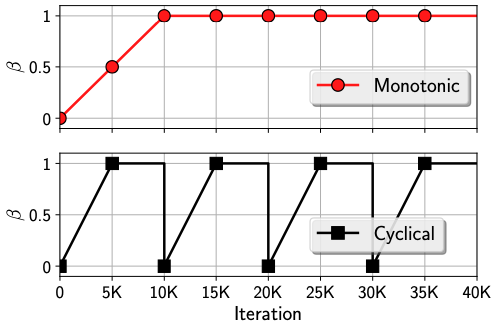
\includegraphics[width=0.5\textwidth]{beta_annealing}
    \caption[Annealing strategy of the KL weight term in variational auto-encoders]{Two annealing strategies for the $\beta$ term that weights the KL divergence in the loss function of variational auto-encoders. The upper graph shows a monotonic increase of $\beta$, the lower graph a cyclical annealing strategy. The picture is from \cite{Fu_Li_Liu_Gao_Celikyilmaz_Carin_2019}.}
    \figlbl{beta_annealing}
\end{figure}


In this thesis, $4$ variational auto-encoders are used. Each VAE consists of an encoder, two fully-connected layers to calculate $\boldsymbol{\mu}$ and $\boldsymbol{\sigma}$, and a decoder.
The encoder consists of $3$  convolutional layers with $32$, $64$, and $128$ channels. Each convolutional layer has a stride of $2$, halving the size of the input in each layer.
The decoder has the inverse structure of the encoder, i.e. $3$ convolutional layers with $128$, $64$, and $32$ channels.
The fully connected layer for predicting $\boldsymbol{\mu}$ and $\boldsymbol{\sigma}$ have $32$ neurons.
The network architecture is shown in Figure \figref{horizontal_org_arch1}.


\begin{figure}[h]
    \centering
    \resizebox{0.99\textwidth}{!}
{
\begin{tikzpicture}
\tikzstyle{connection}=[ultra thick,every node/.style={sloped,allow upside down},draw=\edgecolor,opacity=0.7]
\tikzstyle{copyconnection}=[ultra thick,every node/.style={sloped,allow upside down},draw={rgb:blue,4;red,1;green,1;black,3},opacity=0.7]


\node[canvas is zy plane at x=0] (input) at (0,0,0) {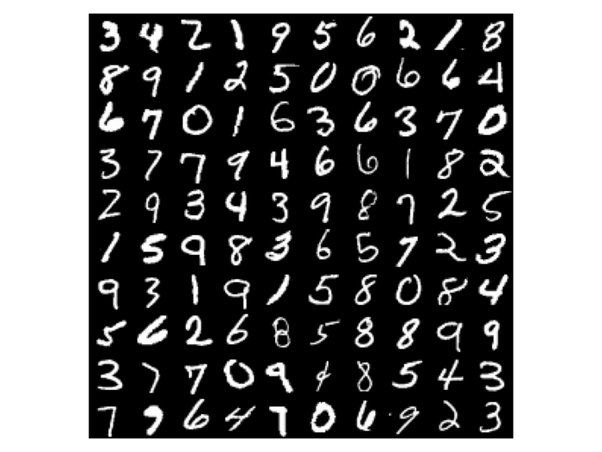
\includegraphics[width=8cm,height=8cm]{imgs/mnist.jpeg}};


\pic[shift={(3,0,0)}] at (input) 
    {Box={
        name=conv1,
        caption=Conv + ReLU,
        xlabel={{1, }},
        zlabel=32,
        fill=\ConvColor,
        height=20,
        width=2,
        depth=20
        }
    };


\draw [connection]  (input) ++(0,0,0)    -- node {\midarrow} (conv1-west);


\pic[shift={(2,0,0)}] at (conv1-east) 
    {Box={
        name=conv2,
        caption=Conv + ReLU,
        xlabel={{32, }},
        zlabel=64,
        fill=\ConvColor,
        height=12,
        width=4,
        depth=12
        }
    };


\draw [connection]  (conv1-east)    -- node {\midarrow} (conv2-west);


\pic[shift={(2,0,0)}] at (conv2-east) 
    {Box={
        name=conv3,
        caption=Conv + ReLU,
        xlabel={{64, }},
        zlabel=128,
        fill=\ConvColor,
        height=6,
        width=6,
        depth=6
        }
    };


\draw [connection]  (conv2-east)    -- node {\midarrow} (conv3-west);


\pic[shift={(2,2,0)}] at (conv3-east) 
    {Box={
        name=fcn1,
        caption=FC + ReLU,
        xlabel={{" ","dummy"}},
        zlabel=32,
        fill=\SoftmaxColor,
        opacity=0.8,
        height=3,
        width=3,
        depth=6
        }
    };


\pic[shift={(2,-2,0)}] at (conv3-east) 
    {Box={
        name=fcn2,
        caption=FC + ReLU,
        xlabel={{" ","dummy"}},
        zlabel=32,
        fill=\SoftmaxColor,
        opacity=0.8,
        height=3,
        width=3,
        depth=6
        }
    };


\draw [connection]  (conv3-east)    -- node {\midarrow} (fcn1-west);


\draw [connection]  (conv3-east)    -- node {\midarrow} (fcn2-west);


\pic[shift={(2,-2,0)}] at (fcn1-east) 
    {Box={
        name=conv4,
        caption=Conv + ReLU,
        xlabel={{128, }},
        zlabel=64,
        fill=\ConvColor,
        height=6,
        width=6,
        depth=6
        }
    };


\draw [connection]  (fcn1-east)    -- node {\midarrow} (conv4-west);


\draw [connection]  (fcn2-east)    -- node {\midarrow} (conv4-west);


\pic[shift={(2,0,0)}] at (conv4-east) 
    {Box={
        name=conv5,
        caption=Conv + ReLU,
        xlabel={{64, }},
        zlabel=32,
        fill=\ConvColor,
        height=12,
        width=4,
        depth=12
        }
    };


\draw [connection]  (conv4-east)    -- node {\midarrow} (conv5-west);


\pic[shift={(2,0,0)}] at (conv5-east) 
    {Box={
        name=conv6,
        caption=Conv + ReLU,
        xlabel={{32, }},
        zlabel=1,
        fill=\ConvColor,
        height=20,
        width=2,
        depth=20
        }
    };


\draw [connection]  (conv5-east)    -- node {\midarrow} (conv6-west);


\node[canvas is zy plane at x=3] (output) at (conv6-east) {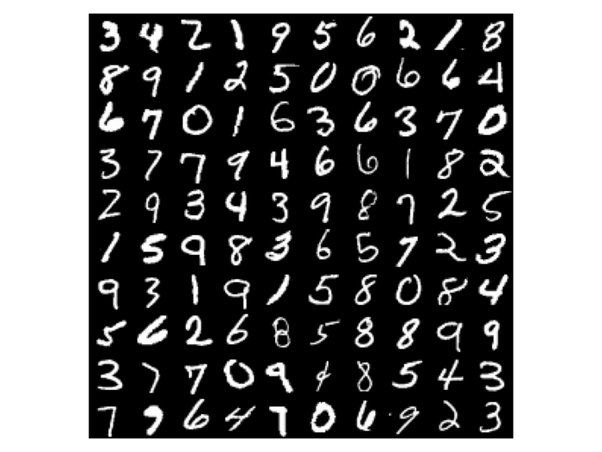
\includegraphics[width=8cm,height=8cm]{imgs/mnist.jpeg}};


\draw [connection]  (conv6-east)     -- node {\midarrow} ($(output) + (0.5,0,0)$);


\end{tikzpicture}
}
    \caption[Architecture of the variational auto-encoder used for horizontal self-organisation]{Architecture of the variational auto-encoder used for horizontal self-organisation.}
    \figlbl{horizontal_org_arch1}
\end{figure}


Each VAE is trained independently with the goal to minimize the loss function as described in \eqref{hso_6}.
Adam \sidecite{Kingma_Ba_2017} is used as optimizer with a learning rate of $1\cdot 10^{-3}$ and the mini-batch size is $32$.






\subsection{Communication}\seclbl{horizontal_self_org_methods_communication}
The VAEs receive patches of the input image and thus have a very limited field-of-view on the image.
Figure \figref{average_sample} visualizes the patches that are fed into the VAEs when the MNIST data set \cite{Lecun_Bottou_Bengio_Haffner_1998} is used.
.....


\begin{figure}[h]
    \centering
    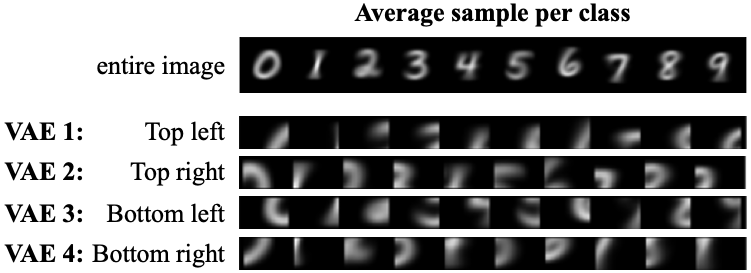
\includegraphics[width=0.99\textwidth]{average_sample}
    \caption[Average sample of the MNIST data set per class]{The average of all samples in the MNIST data set for each class. The first row shows the average of all samples, the 2nd to 5th row the average per patch that is fed into the models.}
    \figlbl{average_sample}
\end{figure}


For many VAEs, some of the digits look similar due to the limited field-of-view. For example, .........
Thus, a VAE cannot decide on its own which digit is depicted in the image.


\subsection{Class Prediction}
% average mu = cluster center -> World model of a digit

\subsubsection{Multiple Prototypes}


\subsubsection{VQ-VAE}
In the case of classification, the latent space has to be shaped in a way that allows to assign a latent representation to a class.
This can be simplified if the encoder maps the input image to a discrete variable in the latent space.
Vector quantised variational auto-encoders (VQ-VAE) \sidecite{NIPS2017_7a98af17} model such a discrete latent space by using vector quantisation (VQ).
Vector quantisation is a method that maps multi-dimensional vectors to a finite set of ``code''-vectors.
An image is fed into the encoder to obtain the encoder output $\boldsymbol{z}_e$.
Afterwards, a nearest neighbor lookup is made to find the code-vector that is most similar to $\boldsymbol{z}_e$.
The code-vector, also called the quantized vector $\boldsymbol{z}_q$ is fed into the decoder to reconstruct the image.





TODO: This has not been implemented yet (therefore, not explained in more detail).


\subsection{Predicting bigger Patches}
Applying a monotonic annealing to the KL divergence weight term $\beta$ is the first measure to improve the latent space distribution.
Another measure is to predict bigger patches.
The VAEs have a very limited field of view and cannot distinguish some of the digits on their own (c.f. \secref{horizontal_self_org_methods_communication}).
However, by predicting bigger patches, the VAEs can be encouraged to better distinguish similar looking patches.
For example, the patches for the digits $xxxxx$ and $xxxxx$ look very similar for the first VAE that receives the patch extracted from the top left corner of the samples.
Since the target prediction of these two digits is similar, they are located closely together in the latent space.
When bigger patches or the entire image is predicted by a VAE, the target predictions of the digits $xxxxx$ and $xxxxx$ become different.
As a consequence, they are not mapped that closely together in the latent space anymore.
Thus, predicting bigger patches helps to push apart latent representations of objects that have a high similarity patch-wise but a low similarity image-wise.


\subsection{Model Heads}



\subsection{Sparsity}








\section{Results}\seclbl{horizontal_self_org_results}







% TODO: Missmatch Biologische Neuronen (binär, spikes, divers, sparse) <-> DL Neuronen (endlos viele Zustände) beschreiben



%TODO: vereinheitliche Mathe: Was ist underline, was ist hochgestellt in Klammern ($z^{(i)}$) und was ist hochgestellt in eckigen Klammern? Bei NN: Was ist n, was ist m, ... (+ Lernraten Symbol, Loss Symbol, etc.)
%Sind alle Vektoren bold?

% TODO: target function und objective function vereinheitlichen
% TODO: net-fragment or net fragment

